\onecolumn
\section{Different types of editing}

\xhdr{Text-based Item Editing.} 
Because the optimized model keeps the memory of the original vocabulary, replacing an item with another one described by a text prompt can be simply achieved by changing the corresponding item prompt to the target text. 
The learned item prompt can also be used along with other words to form a new prompt. 

\xhdr{Image-based Item Editing}
Given two images, to replace an item in the source image with another one in the reference image, all item prompts in both images should be injected into the same model. 
Then the item replacement can be realized by the corresponding prompt replacement.
Note that this setting is more general compared to classical image-based editing scenarios where the reference is an entire image instead of an item.
This is particularly useful when it is hard to find a solo focus reference.


\xhdr{Mask-based Item Editing} 
Besides replacing items by changing the prompt, we can also keep the item semantics but change the appearance of the item in the image by editing the corresponding segmentation mask.
The mask editing includes moving the mask position, resizing mask, refining the mask shape, or redrawing the mask.
Therefore, we consider four types of mask-based editing in the experiment including changing item position, size, shape, and post-editing refinement.


\xhdr{Item Removal}
Items in the image can be removed by deleting the corresponding item mask and item-prompt pair from the image.
The deleted region will be filled by nearby region masks and corresponding item-prompt pairs.

\section{Prompt Interpolation}
Instead of replacing the original item prompt with the target one (image/text guided), we can also interpolate between the two and get the transition results.
As shown in Fig. \ref{sfig::ablate}, we interpolate the embeddings after the text encoder and derive the mixed embedding using $c =\text{alpha}\cdot c_{\text{guide}} + (1-\text{alpha})\cdot c_{\text{orig}}$.

\begin{figure*}[h]
  \centering 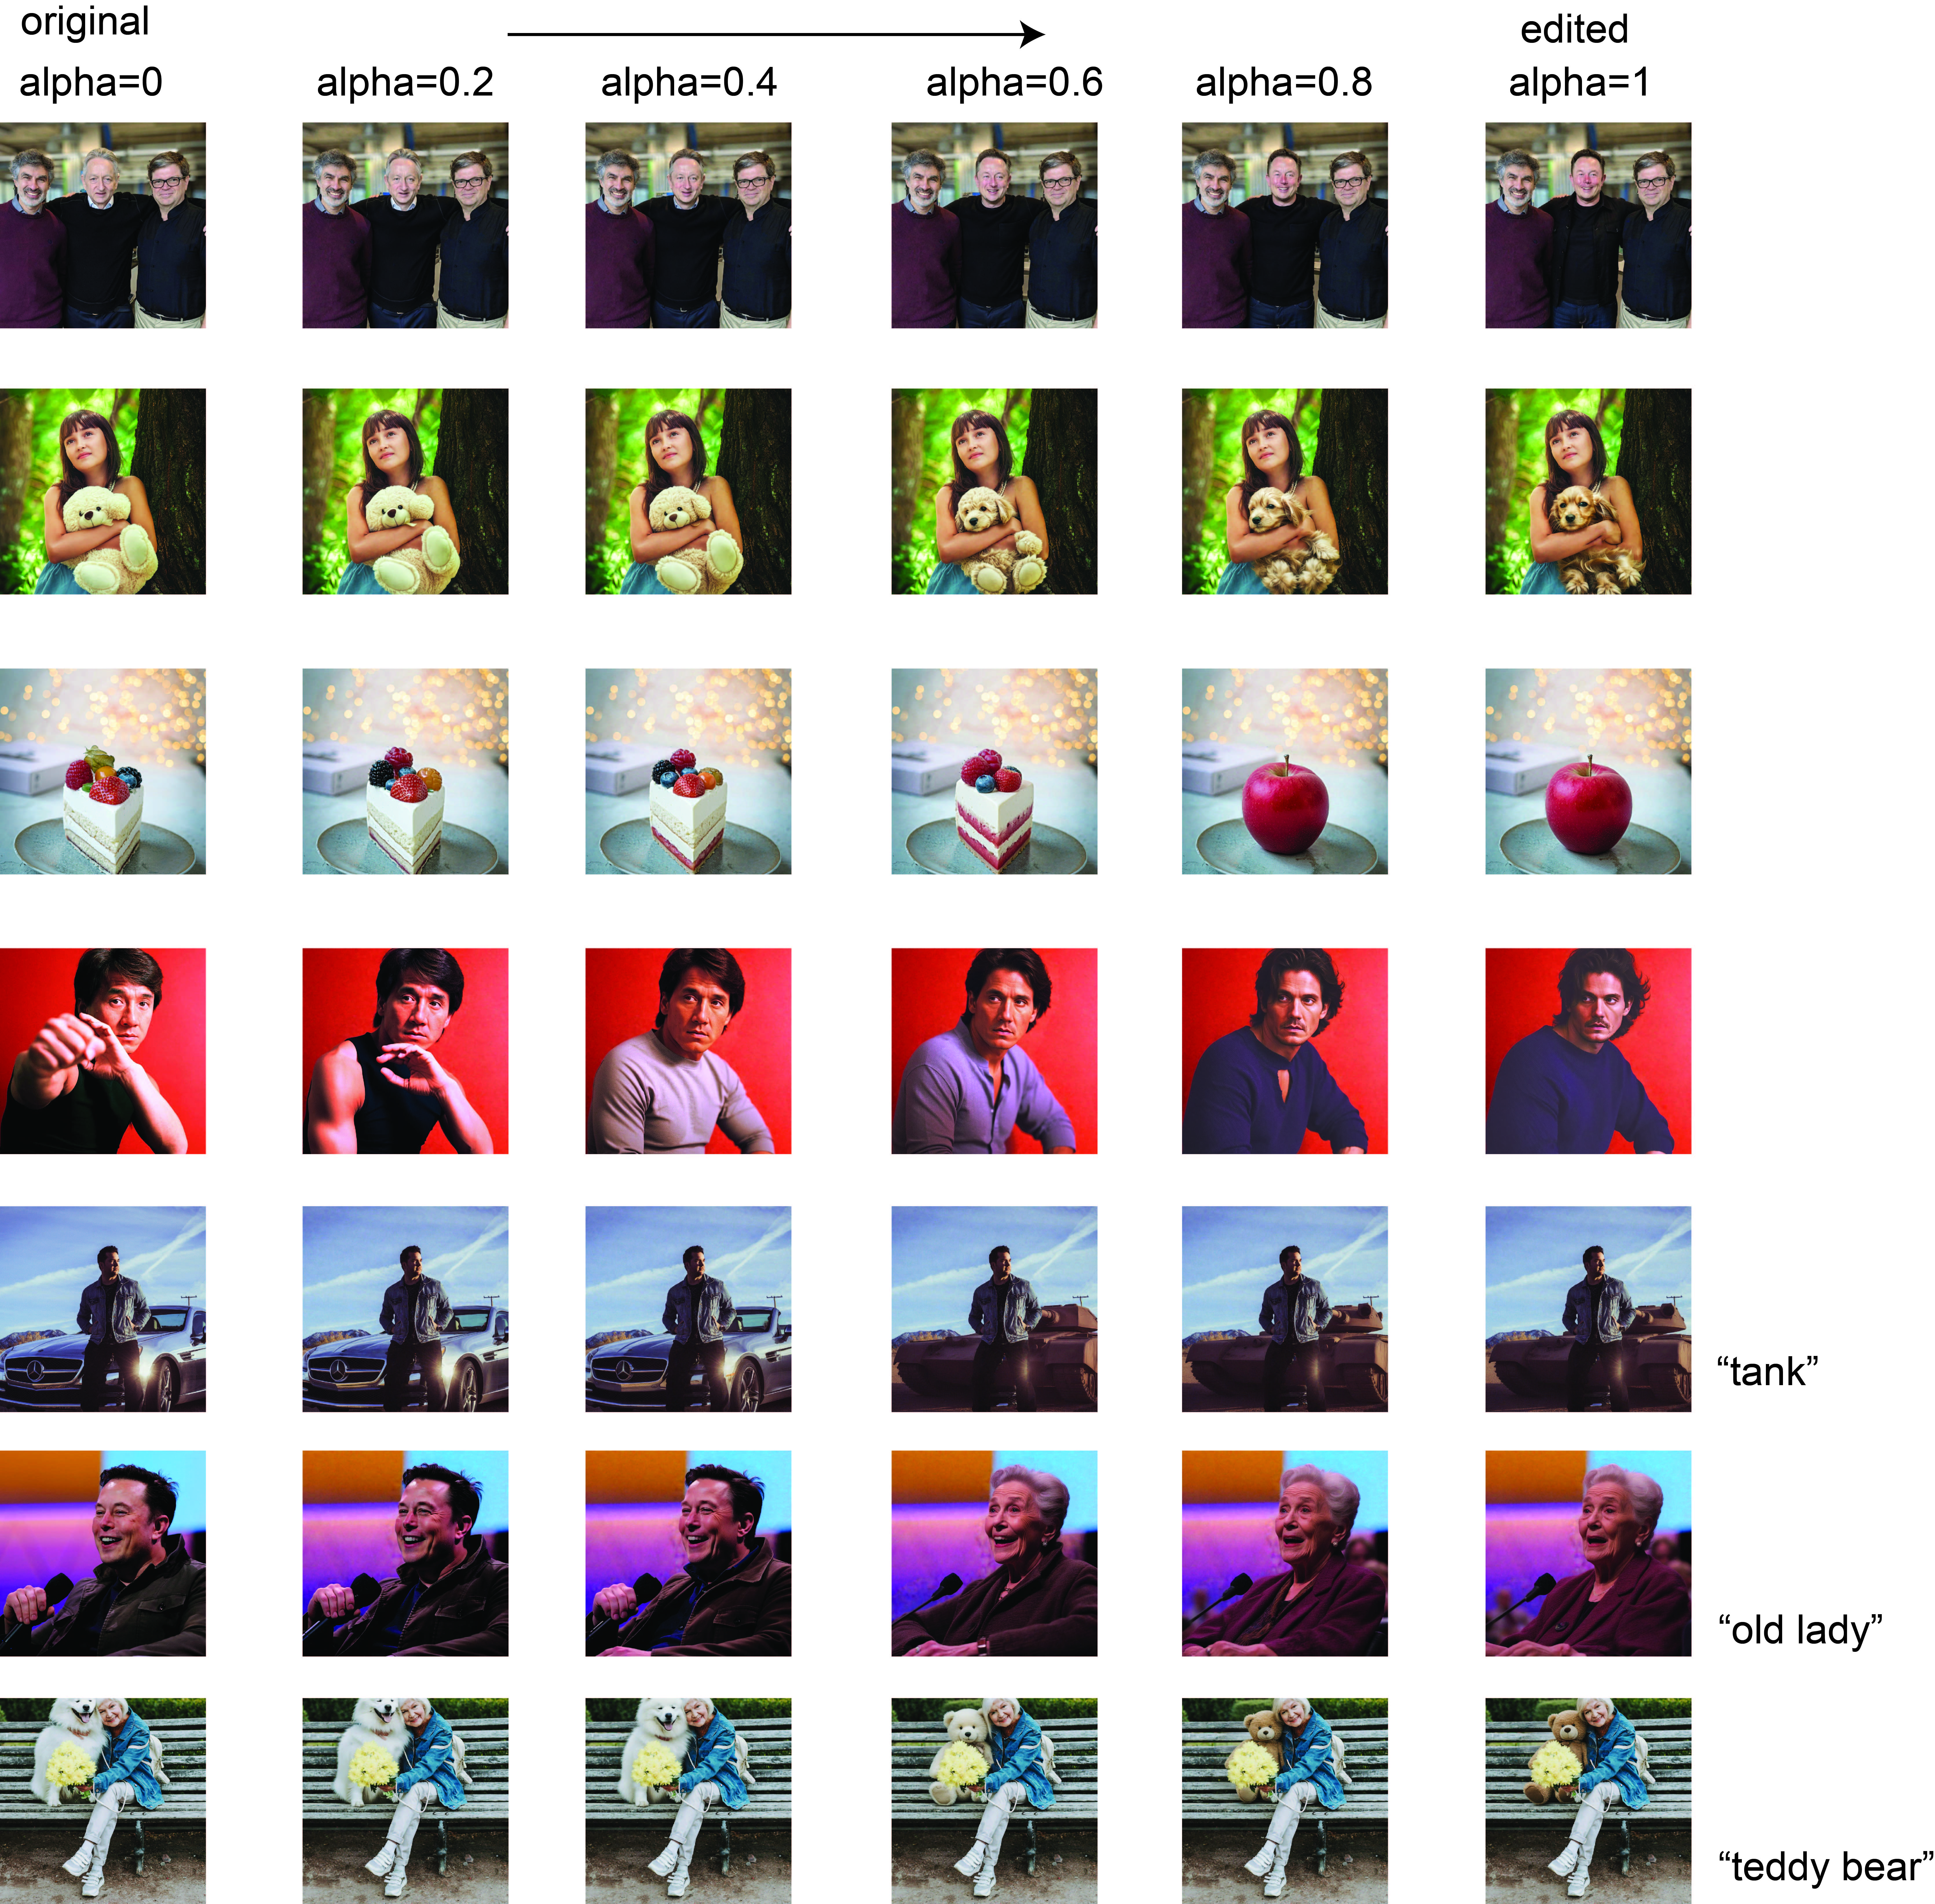
\includegraphics[width=0.8\linewidth]{fig/appendix_fig2_small.jpg}
  \caption{
  Mixing of the original and guidance images by linearly interpolating the embeddings of the two.
  }
  \label{sfig::ablate}
\end{figure*}
\clearpage

\section{More Text-Based Editing}
\begin{figure*}[h]
  \centering 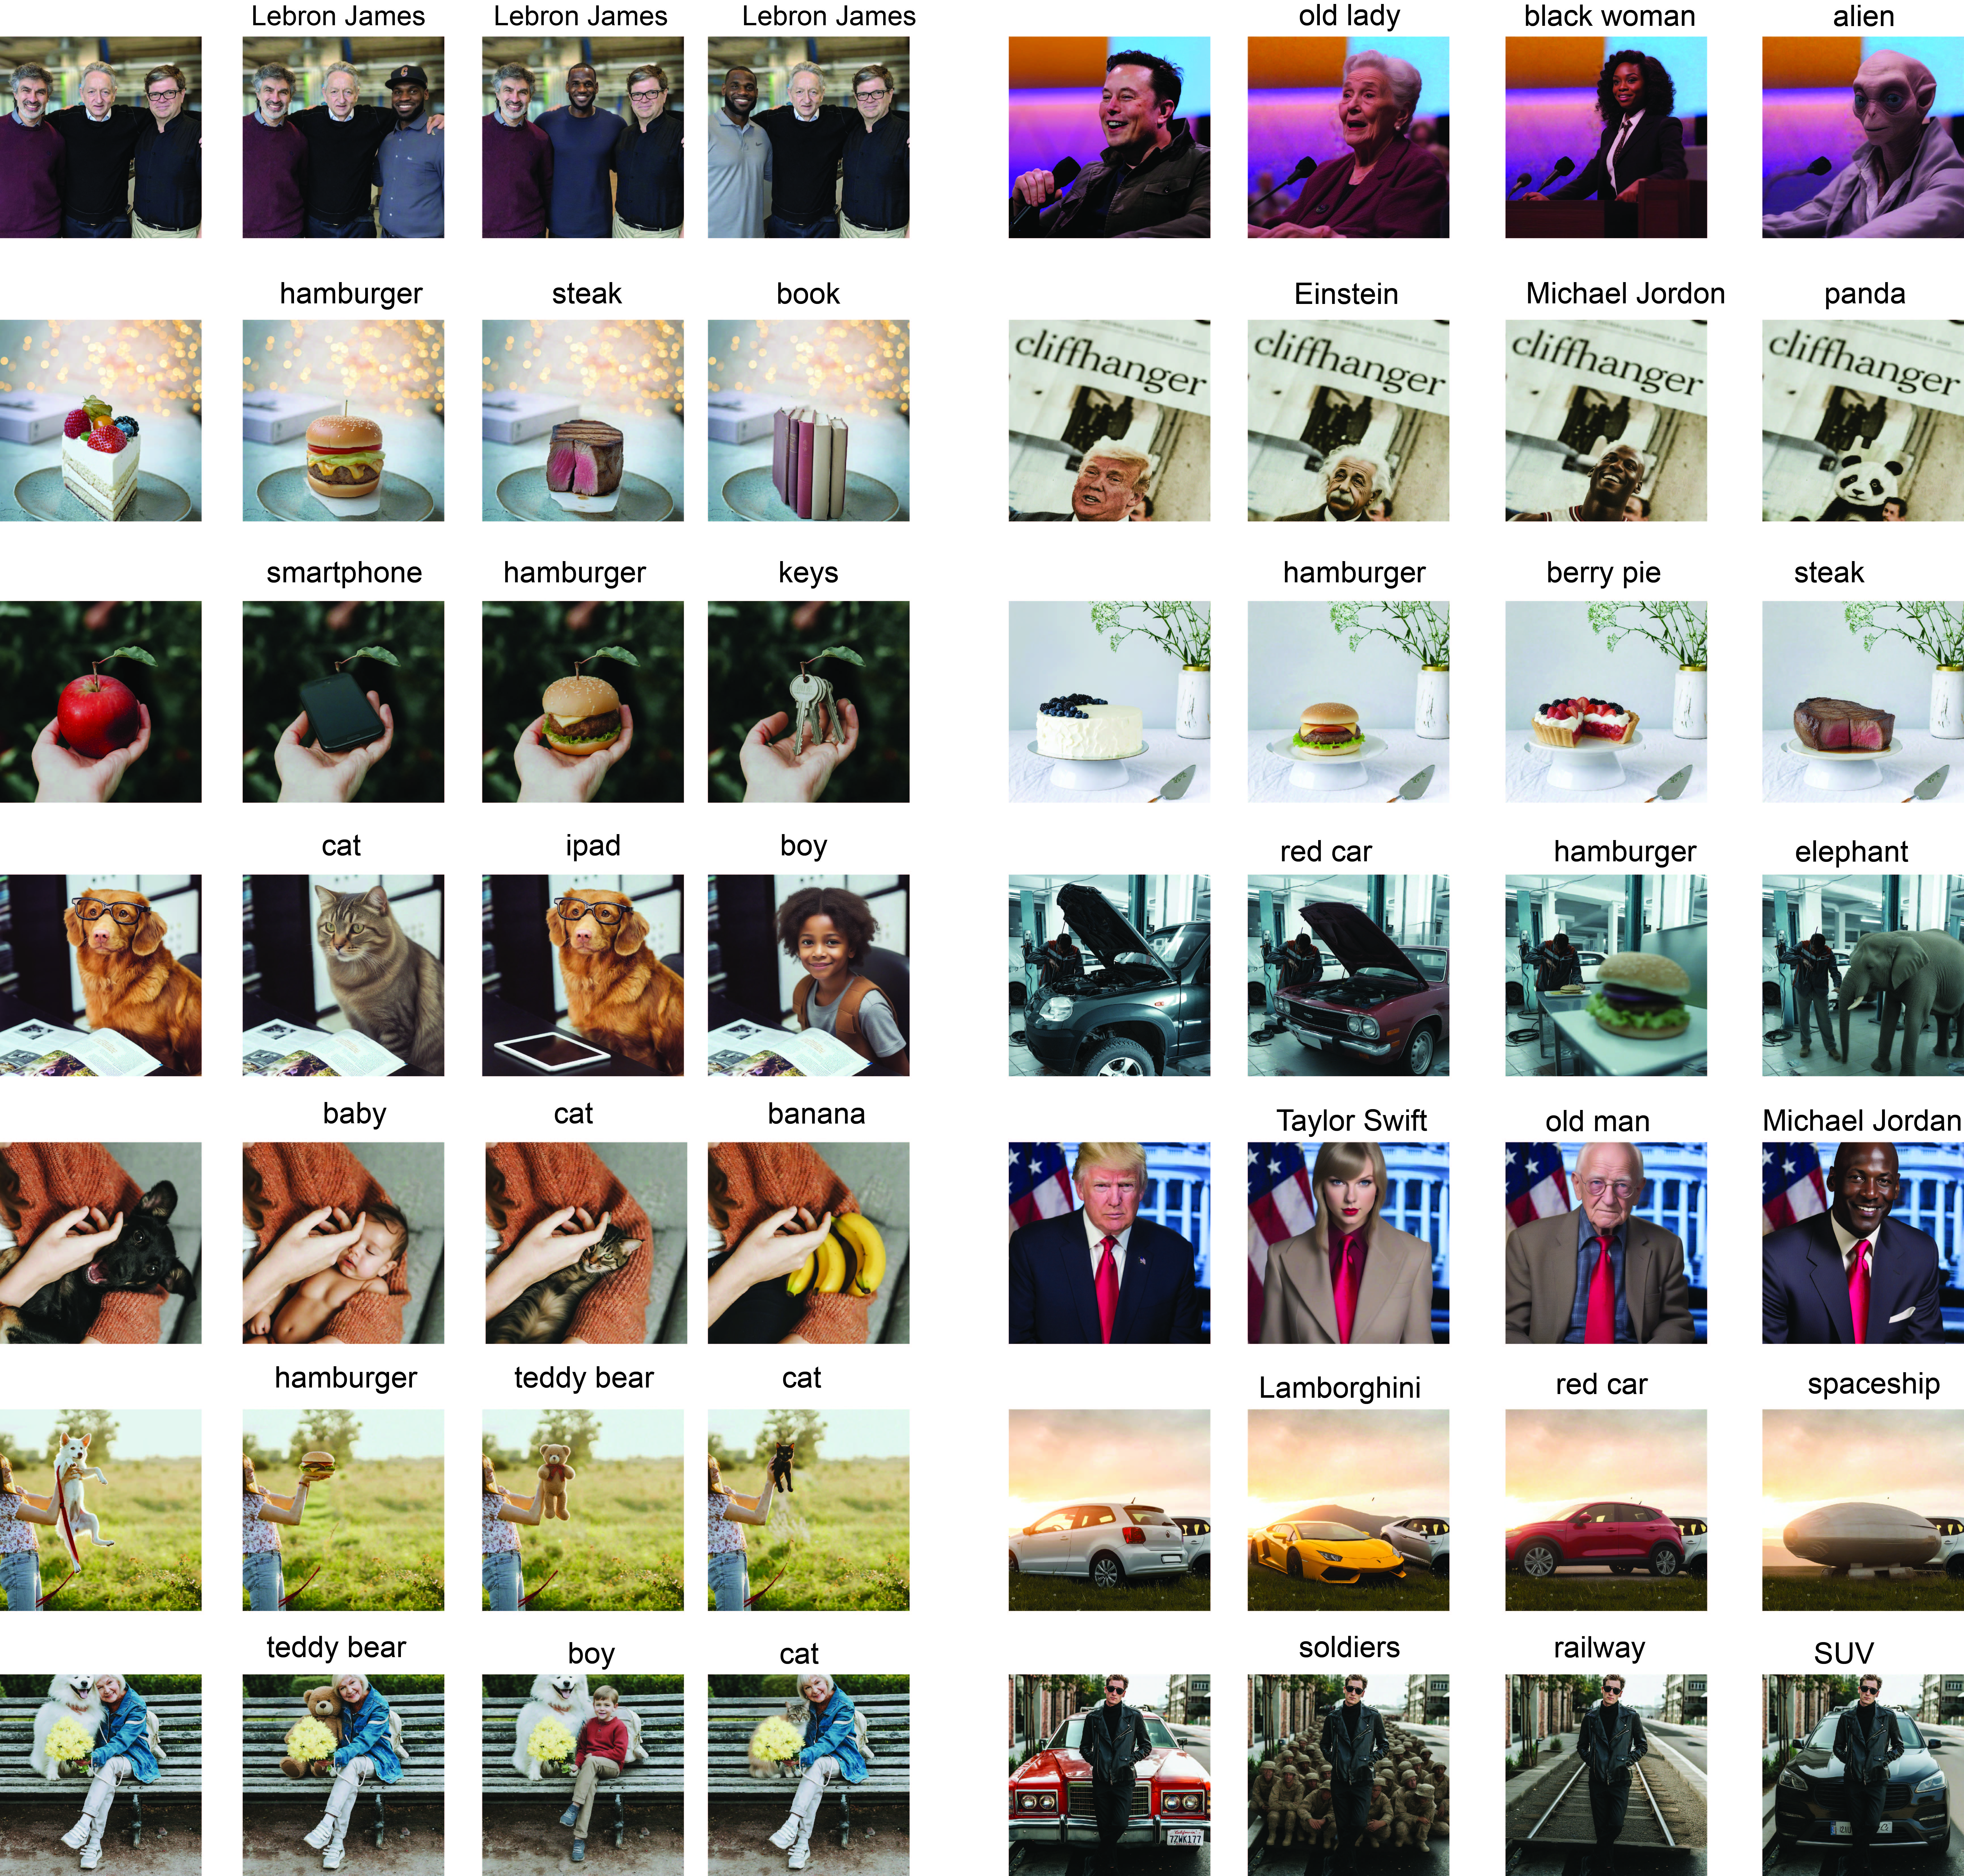
\includegraphics[width=0.8\linewidth]{fig/appendix_fig0_small.jpg}
  \caption{
  More text-editing results of replacing one item with target prompts.
  }
  \label{sfig::text}
\end{figure*}

\clearpage
\section{More Image-Based Editing}
As marked in Fig. \ref{sfig::img}, several failure examples occur: 
(1) \textbf{Color is harder to learn than shape}: in the Lamborghini example $a$, the shape is preserved while the yellow color is lost.
(2) \textbf{Item should have clear meanings}: in the man-in-car example $b$, because the man picture through the window is blurred and DPM cannot understand, the inpainting results will be unnatural.
(3) \textbf{Out-of-domain image is hard to learn}:
In the celebrity face example $c$, if the celebrity face is not natural or highly Photoshopped, it will be hard for DPMs to reconstruct it and therefore lead to weird face results.



\begin{figure*}[h]
  \centering 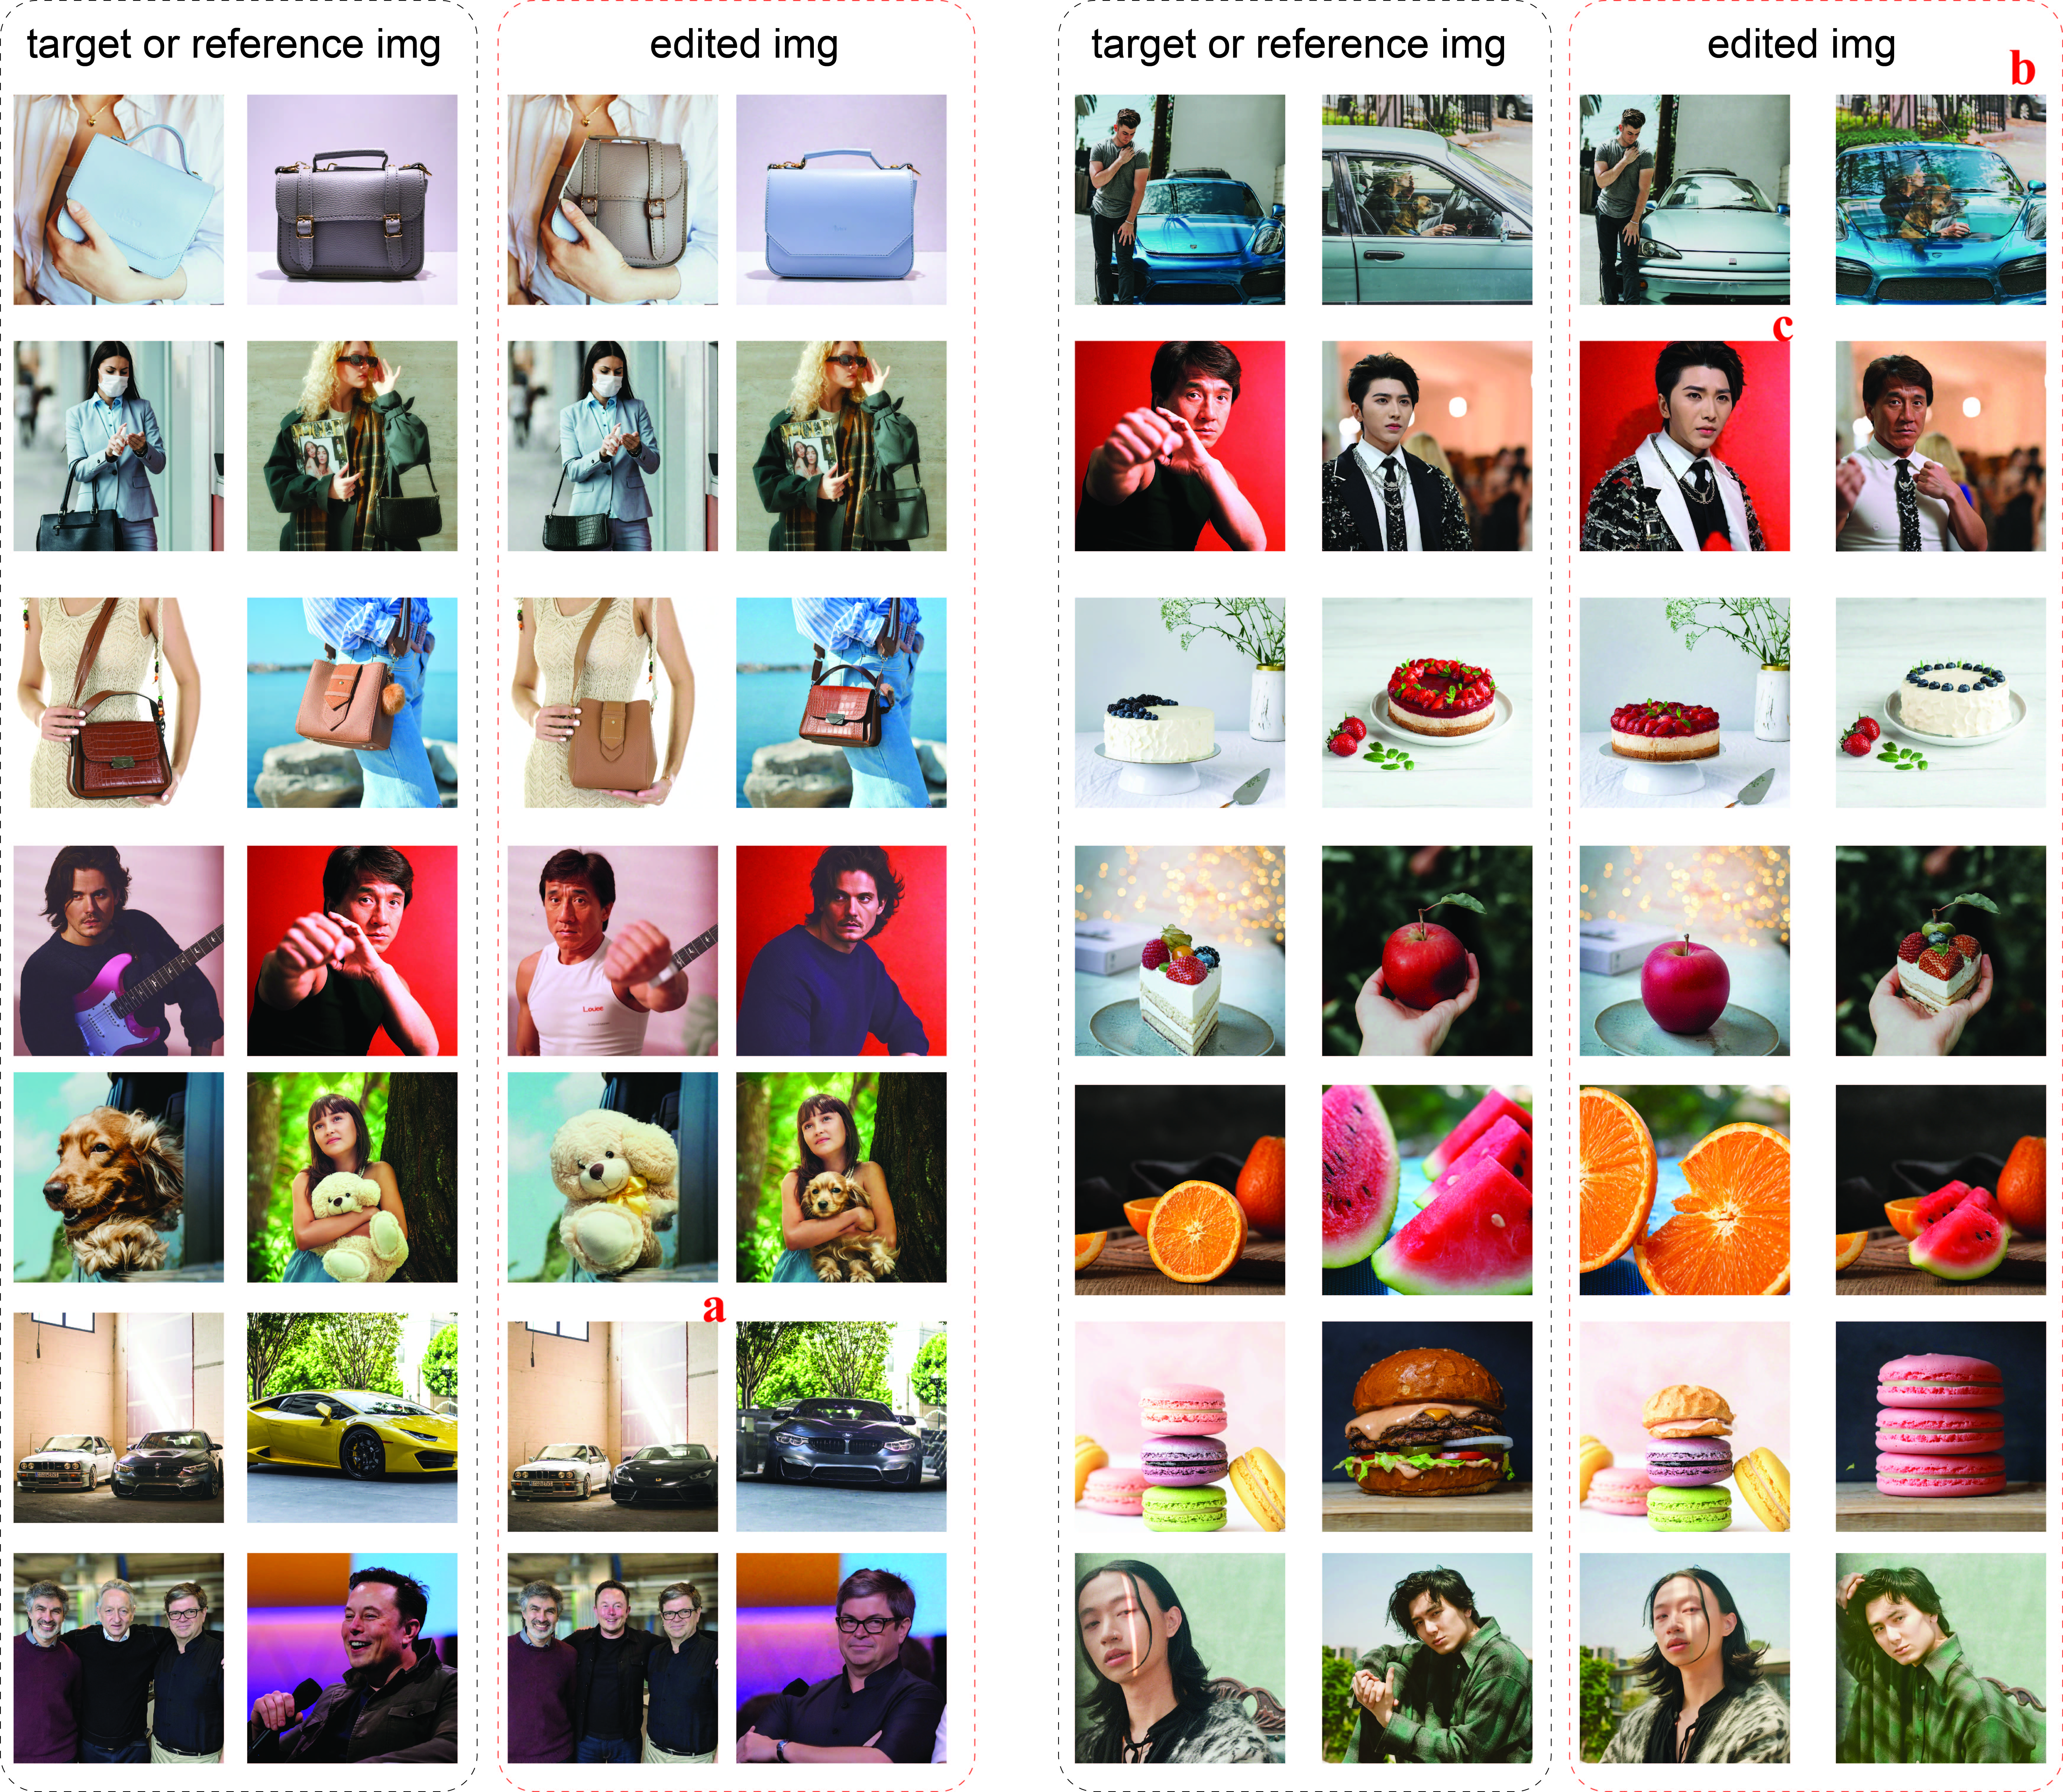
\includegraphics[width=0.8\linewidth]{fig/appendix_fig1_small.jpg}
  \caption{
  More image-guided editing results of replacing one item with the reference item.
  Failure examples are marked by red letters.
  }
  \label{sfig::img}
\end{figure*}



